\section{Problem Set 1}
\subsection{Problem 1: Your Mission, Your Challenge}

In this section of the report, we examine several different mission formats with the goal of choosing one to work on for the project.

\subsubsection{Mission 1: VISORS (VIrtual Super-resolution Optics with Reconfigurable Swarms)}

\paragraph{Mission Name and Operator:} VISORS, which is a multi-institution collaboration with the GN\&C subsystem developed and operated by Stanford's Space Rendezvous Laboratory.

\paragraph{Primary and Secondary Mission Objectives:}
\begin{itemize}
    \item Primary: Obtain images of active regions of the Sun's coronal area in the extreme ultraviolet spectrum with unprecedented resolution; with the goal of improving the current thermodynamic models of the solar corona.
    \item Secondary: Demonstrate capabilities of novel convex optimization-based model predictive control algorithms with no flight heritage, as well as higher accuracy autonomous control. 
\end{itemize}

\paragraph{Number and Type of Satellites:} 
Two 6U CubeSats, one of which contains the optical payload, and the other which contains the detector.

\paragraph{Absolute and Relative Orbit Parameters:}
\begin{itemize}
    \item Low Earth Orbit (LEO)
    \item Sun-synchronous orbit
    \item Therefore roughly: [$a = 6978$ km, $e = 0.001$, $i = 97.8^{\circ}$, $\Omega = \text{tbd}$, $\omega = \text{tbd}$, $M = \text{tbd}$]
    \item Relative configuration: Two spacecraft flying in formation with 40 meters separation, maintaining millimeter level accuracy.
    \item Launch date: Originally scheduled for October 2024 (now 2026)
    \item Mission duration: 100 observation attempts divided into 10 sets of 10 observations, with 2 weeks in standby mode between sets of observations.
\end{itemize}

\paragraph{Basic Description of Functioning/Scientific Principle:}
VISORS optics spacecraft has a photon sieve payload that uses constructive interference on a detector payload that's on the detector spacecraft to focus light. This creates a high contrast image with 0.1" resolution in the extreme ultraviolet. The spacecraft also has deployable solar panels that double as sunshade. These help block light coming from outside the area of interest.

\paragraph{Key DGN\&C Requirements:}
\begin{itemize}
    \item \textbf{Alignment with active region (pointing):} The center of the photon sieve must not deviate from the line connecting the center of the detector aperture and the target active region by more than 18 mm.
    \item \textbf{Line-of-sight stability/image drift:} The spacecraft's inertial relative velocity in the plane perpendicular to the line of sight must not exceed 0.2 mm/s, so common features can be tracked across exposures.
    \item \textbf{Focus:} The distance between the detector aperture center and the photon sieve pattern center must not deviate by more than 15 mm from the nominal separation of 40 m.
\end{itemize}

\paragraph{Classification of DSS:}
Formation-flying mission with high-precision relative positioning requirements.

\subsubsection{Mission 2: TanDEM-X (TerraSAR-X Add-on for Digital Elevation Measurement)}

\paragraph{Mission Name and Operator:} 
TanDEM-X, operated by the German Aerospace Center (DLR) and Airbus Defence and Space.

\paragraph{Primary and Secondary Mission Objectives:}
\begin{itemize}
    \item Primary: Generate a consistent global Digital Elevation Model (DEM) corresponding to the HRTE-3 model specifications with a relative vertical accuracy of 2 m for flat terrain and 4 m for steep terrain.
    \item Secondary: Demonstrate advanced SAR imaging techniques and interferometric satellite formation in space.
\end{itemize}

\paragraph{Number and Type of Satellites:} 
Two identical X-band radar satellites (TerraSAR-X and TanDEM-X).

\paragraph{Absolute and Relative Orbit Parameters:}
\begin{itemize}
    \item Sun-synchronous orbit at 514 km altitude
    \item 97.44$^{\circ}$ inclination
    \item 11-day repeat cycle (167 orbits)
    \item Eccentricity: 0.001
    \item Therefore roughly: [$a = 6892$ km, $e = 0.001$, $i = 97.44^{\circ}$, $\Omega = \text{tbd}$, $\omega = \text{tbd}$, $M = \text{tbd}$]
    \item Relative configuration: Helix formation with typical separation of 200-500 m
    \item Launch dates: TerraSAR-X (June 15, 2007), TanDEM-X (June 21, 2010)
    \item Mission duration: Initially 3 years, extended multiple times (still operational)
\end{itemize}

\paragraph{Basic Description of Functioning/Scientific Principle:}
TanDEM-X operates as a single-pass radar interferometer where two satellites fly in close formation, enabling bistatic SAR interferometry. By precisely measuring the phase difference between radar signals reflected from the Earth's surface to both satellites, the system creates highly accurate elevation maps. The tandem configuration enables highly accurate single-pass cross-track interferogram without the inherent accuracy limitation imposed by repeat pass interferometry due to decorrelation and atmospheric disturbances.

\paragraph{Key DGN\&C Requirements:}
\begin{itemize}
    \item Helix formation control with 150-500 m separation for collision avoidance
    \item Baseline determination with mm-level accuracy using GPS measurements
    \item Phase synchronization between radar instruments with accuracy of ~1º
    \item Automated formation-keeping with daily in-plane maneuvers
    \item Precise relative position knowledge to support bistatic interferometry
\end{itemize}

\paragraph{Classification of DSS:}
Formation-flying mission with meter-level relative positioning requirements.

\subsubsection{Mission 3: Starling}

\paragraph{Mission Name and Operator:} 
Starling, operated by NASA Ames Research Center with the Starling Formation-flying Optical eXperiment (StarFOX) operated by Stanford's Space Rendezvous Laboratory.

\paragraph{Primary and Secondary Mission Objectives:}
\begin{itemize}
    \item Primary: Demonstrate autonomous swarm technologies for distributed space systems, including swarm navigation, maneuver planning, communications and coordination.
    \item Secondary: Demonstrate technologies that enable multipoint science data collection by several small spacecraft flying in swarms.
\end{itemize}

\paragraph{Number and Type of Satellites:} 
Four identical 6U CubeSats built by Blue Canyon Technologies.

\paragraph{Absolute and Relative Orbit Parameters:}
\begin{itemize}
    \item Low Earth Orbit at approximately 550 km altitude
    \item Therefore roughly: [$a = 6928$ km, $e = 0.001$, $i = 97.8^{\circ}$, $\Omega = \text{tbd}$, $\omega = \text{tbd}$, $M = \text{tbd}$]
    \item Relative configuration: Variable distance formation from several kilometers to less than 1 km
    \item Launch date: July 17, 2023 on a Rocket Lab Electron vehicle from New Zealand
    \item Mission duration: Approximately 1 year
\end{itemize}

\paragraph{Basic Description of Functioning/Scientific Principle:}
The Starling mission tests four key technologies: (1) StarFOX (Starling Formation-flying Optical eXperiment), which uses onboard star tracker cameras for swarm navigation, (2) Distributed Spacecraft Autonomy (DSA), which enables the swarm to sense and react to the environment autonomously, (3) inter-satellite communications for networking between spacecraft, and (4) autonomous maneuver planning and execution. The StarFOX system uses an advanced algorithm that processes star tracker images to compute spacecraft orientation and visually detect and track other spacecraft in the swarm. These measurements are then shared between spacecraft, enabling the swarm to determine its position without relying on external navigation sources.

\paragraph{Key DGN\&C Requirements:}
\begin{itemize}
    \item Autonomous angles-only navigation using star tracker cameras
    \item Real-time inter-satellite communications to share measurement data
    \item Distributed orbit determination among all spacecraft
    \item Autonomous collision avoidance and maneuver planning
    \item Cooperative swarm decision-making without ground intervention
\end{itemize}

\paragraph{Classification of DSS:}
Swarm mission with autonomous coordination capabilities and moderate relative positioning requirements (meter to kilometer-level).

\subsubsection{Mission 4: SpaceX Dragon ISS Docking Mission}

\paragraph{Mission Name and Operator:} 
SpaceX Crew Dragon ISS Docking Mission, operated by SpaceX in partnership with NASA.

\paragraph{Primary and Secondary Mission Objectives:}
\begin{itemize}
    \item Primary: Transport crew and/or cargo to and from the International Space Station
    \item Secondary: Demonstrate autonomous rendezvous and docking capabilities
\end{itemize}

\paragraph{Number and Type of Satellites:} 
Two spacecraft (Dragon capsule and International Space Station).

\paragraph{Absolute and Relative Orbit Parameters:}
\begin{itemize}
    \item ISS orbit: $\sim$400-420 km altitude
    \item 51.6° inclination
    \item 90-minute orbital period
    \item Therefore roughly: [$a = 6780$ km, $e = 0.0006$, $i = 51.6^{\circ}$, $\Omega = \text{tbd}$, $\omega = \text{tbd}$, $M = \text{tbd}$]
    \item Relative configuration: Approach from phasing orbit to final docking
    \item Launch dates: Multiple missions since 2020 (Demo-2, Crew-1, Crew-2, ..., Crew-10)
    \item Mission duration: Typically 6 months for crew rotation missions
\end{itemize}

\paragraph{Basic Description of Functioning/Scientific Principle:}
The Dragon spacecraft performs a multi-phase rendezvous with the ISS, including initial phasing, height adjustment maneuvers, coelliptic approach, proximity operations, and final docking. The vehicle uses a combination of absolute and relative navigation sensors to guide it from the initial orbital insertion to the final soft-capture and hard-capture with the ISS docking adapter. The mission requires precise coordination between the approaching vehicle and the target space station.

\paragraph{Key DGN\&C Requirements:}
\begin{itemize}
    \item Far-field rendezvous using absolute navigation (GPS)
    \item Near-field proximity operations using relative navigation (lidar, cameras)
    \item Centimeter-level precision for final docking phase
    \item Autonomous trajectory planning with collision avoidance capabilities
    \item Real-time fault detection and response
    \item Precise attitude control during all mission phases
\end{itemize}

\paragraph{Classification of DSS:}
Rendezvous and docking mission with extremely high precision requirements in the final approach phase (cm-level positioning, mm-level rates).

\subsubsection{Selected Mission for Course Project}
From these candidates, we selected the \textbf{SpaceX Dragon ISS Docking Mission} as the framework for the course project. This was chosen due to our desire to work on the rendezvous problem.

\subsection{Orbit Simulation, Review of Astrodynamics}
\subsubsection{Initial Orbital Elements}

\begin{table}[H]
    \centering
    \begin{tabular}{cccccc} \hline
        $a$ (m) & $e$ & $i$ (deg) & $\Omega$ (deg) & $\omega$ (deg) & $M$ (deg) \\ \hline 
         6780000 & 0.0006 & 51.6 & 0 & 0 & 0 \\ \hline
    \end{tabular}
    \caption{Initial classical orbit elements for the ISS/Dragon mission}
    \label{tab:iss_ics}
\end{table}

\subsubsection{Initial Position and Velocity in ECI Frame}
\begin{align}
    \vec{r}_{ECI} &= [6775932.00, 0.00, 0.00]^T \text{ m} \\
    \vec{v}_{ECI} &= [0.00, 4765.51, 6012.58]^T \text{ m/s}
\end{align}

\subsubsection{Numerical Integration Results}

\begin{figure}[H]
    \centering
    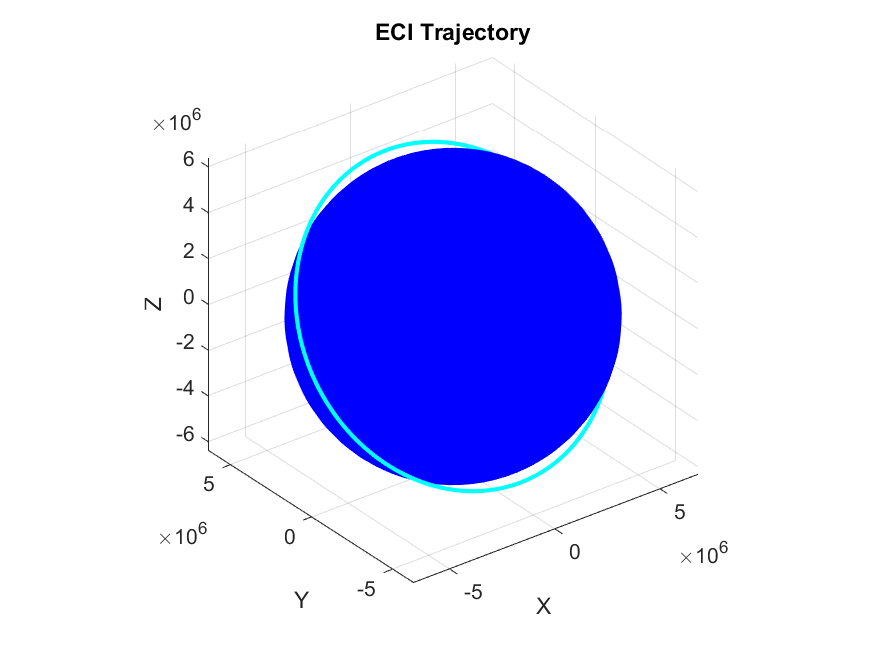
\includegraphics[width=0.5\textwidth]{PS1/Figures/eci_trajectory_unperturbed.png}
    \caption{ECI trajectory without J2 perturbation}
    \label{fig:eci_unperturbed}
\end{figure}

\begin{figure}[H]
    \centering
    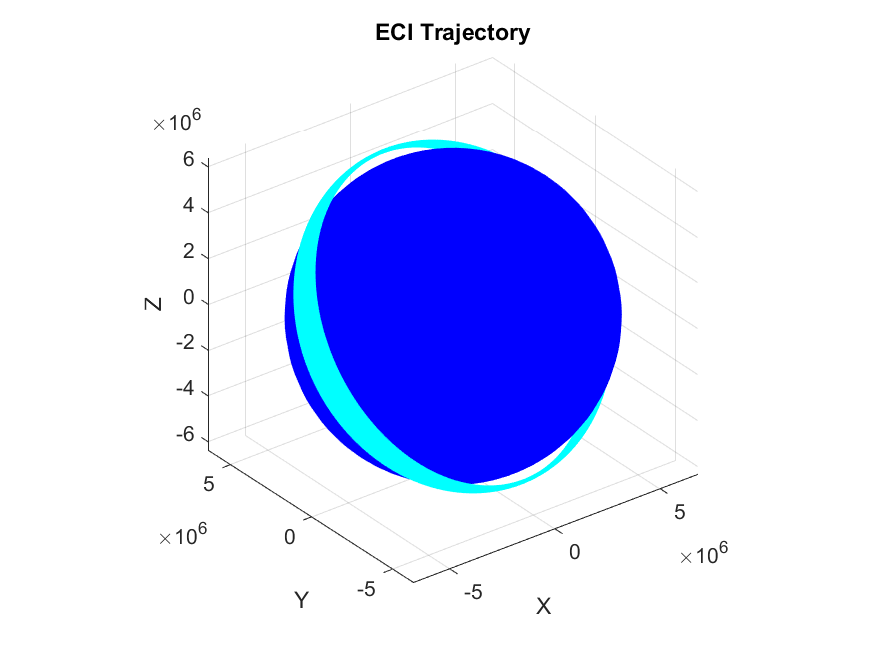
\includegraphics[width=0.5\textwidth]{PS1/Figures/eci_trajectory_j2.png}
    \caption{ECI trajectory with J2 perturbation}
    \label{fig:eci_j2}
\end{figure}

The J2-perturbed trajectory shows a slight precession of the orbital plane, visible as a spreading of the trajectory when compared to the unperturbed case.

\subsubsection{Verification of Numerical Integration}

\begin{figure}[H]
    \centering
    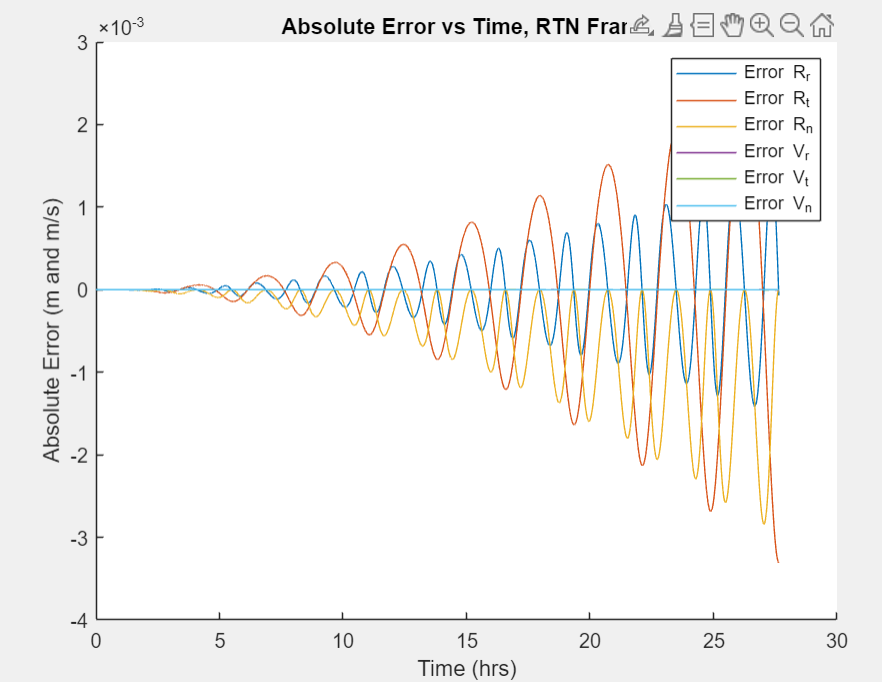
\includegraphics[width=0.5\textwidth]{PS1/Figures/error_comparison.png}
    \caption{Position and velocity errors between numerical integration and analytical solution in RTN frame}
    \label{fig:error_comparison}
\end{figure}

The error comparison shows differences growing to several kilometers over the simulation period, showing accumulated numerical integration errors as expected.

\subsubsection{Orbital Elements and Conservation Properties}

\begin{figure}[H]
    \centering
    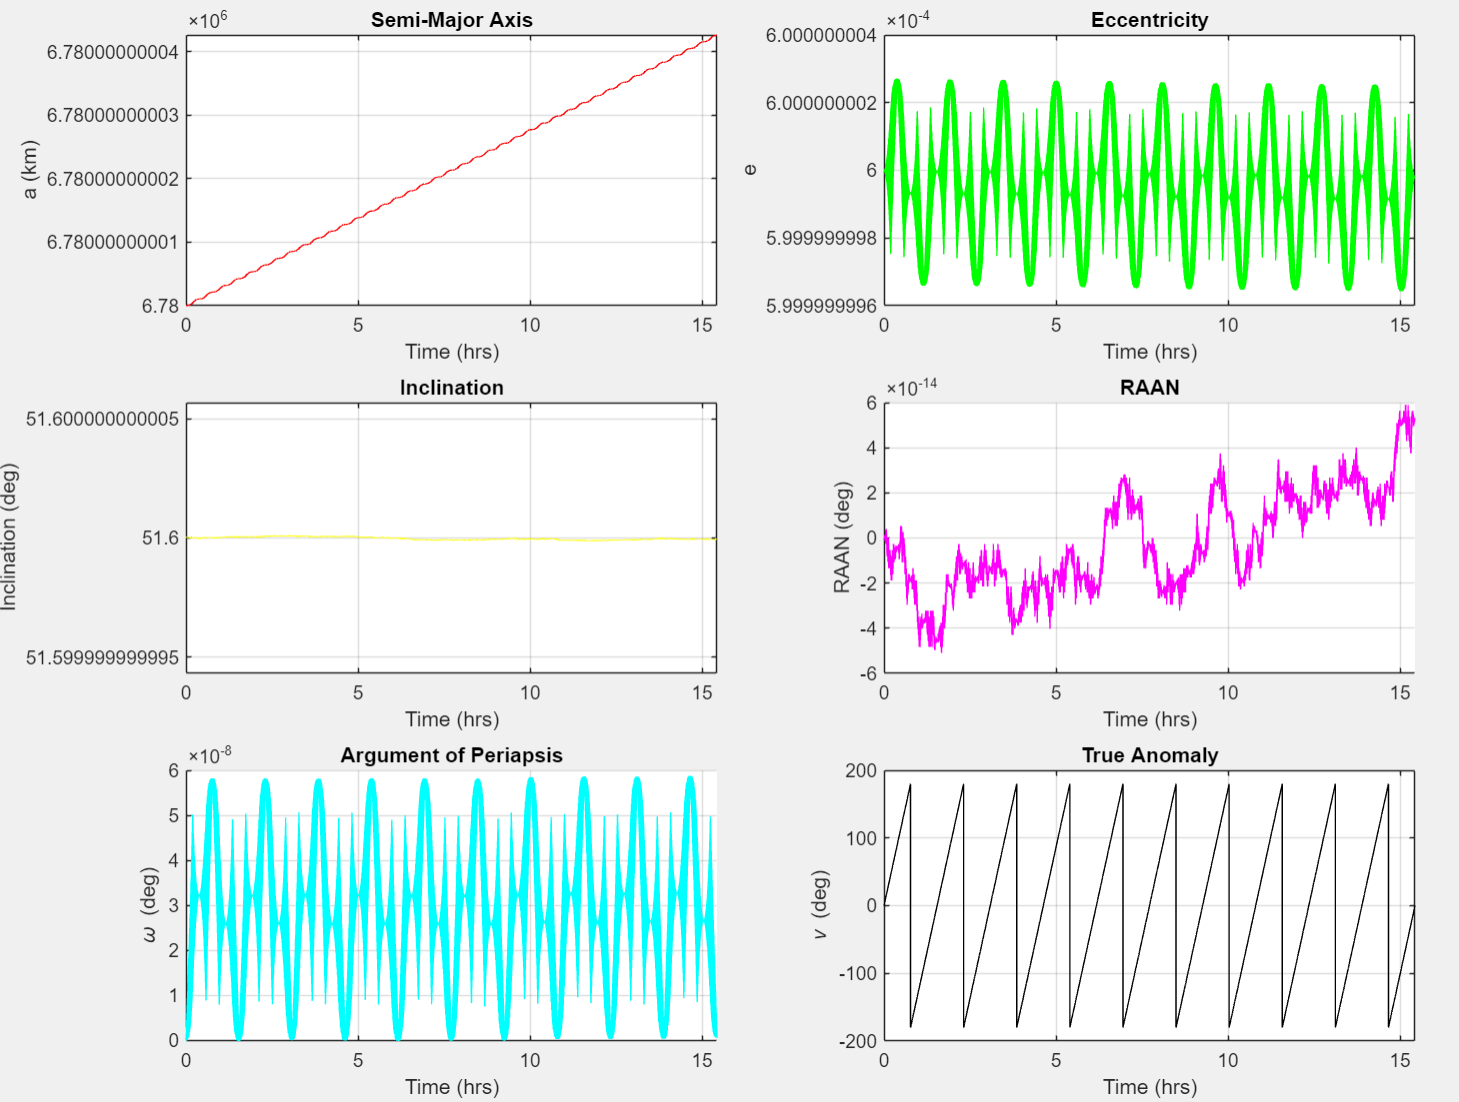
\includegraphics[width=0.5\textwidth]{PS1/Figures/orbital_elements_unperturbed.png}
    \caption{Osculating orbital elements without J2 perturbation}
    \label{fig:oe_unperturbed}
\end{figure}

\begin{figure}[H]
    \centering
    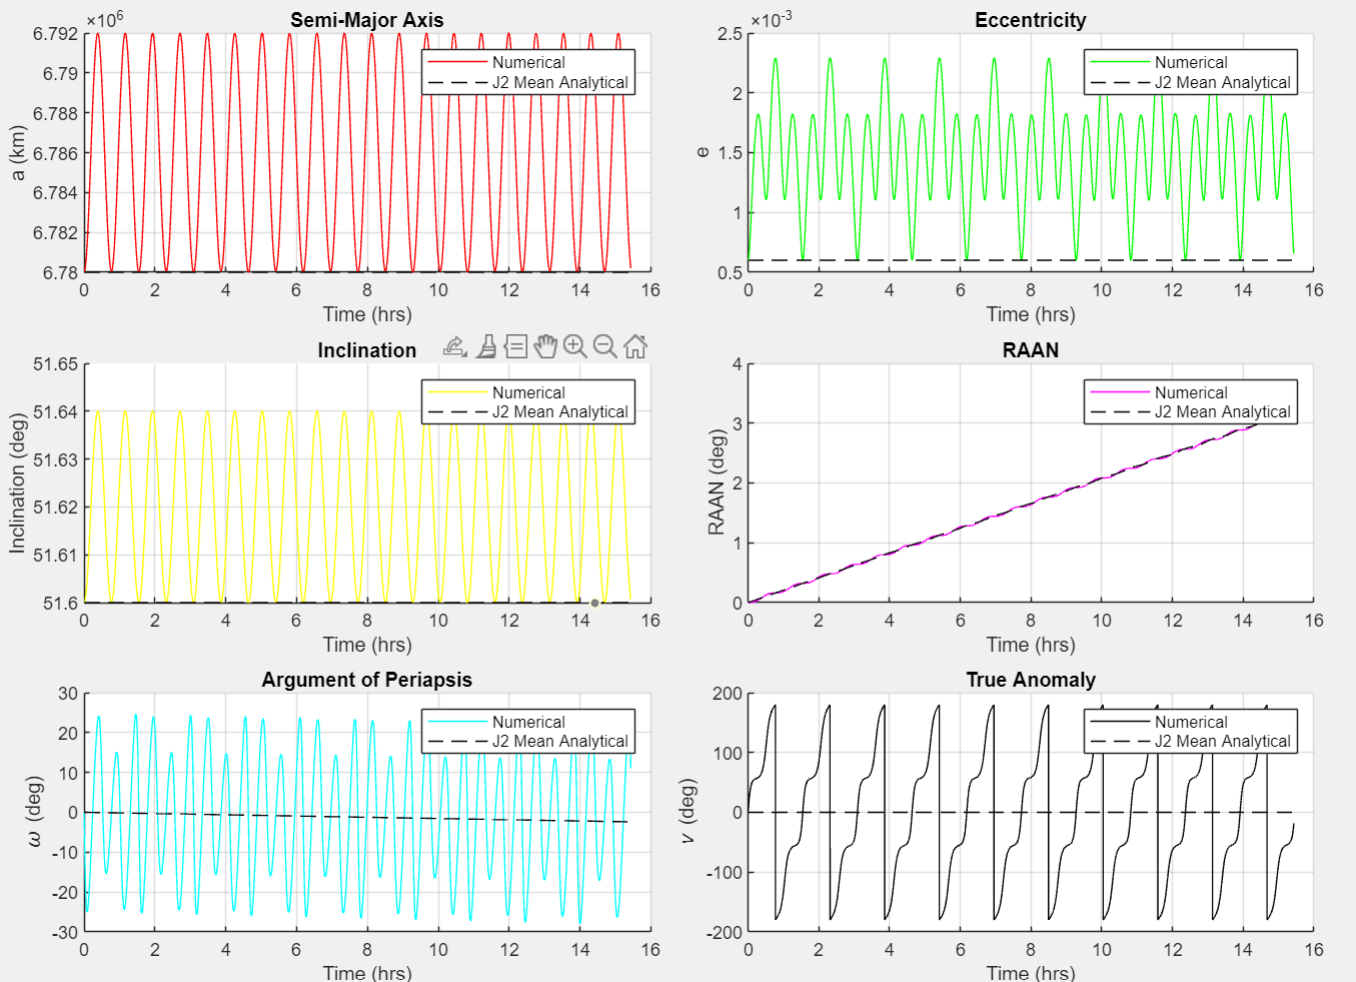
\includegraphics[width=0.5\textwidth]{PS1/Figures/orbital_elements_j2.png}
    \caption{Osculating orbital elements with J2 perturbation}
    \label{fig:oe_j2}
\end{figure}

\begin{figure}[H]
    \centering
    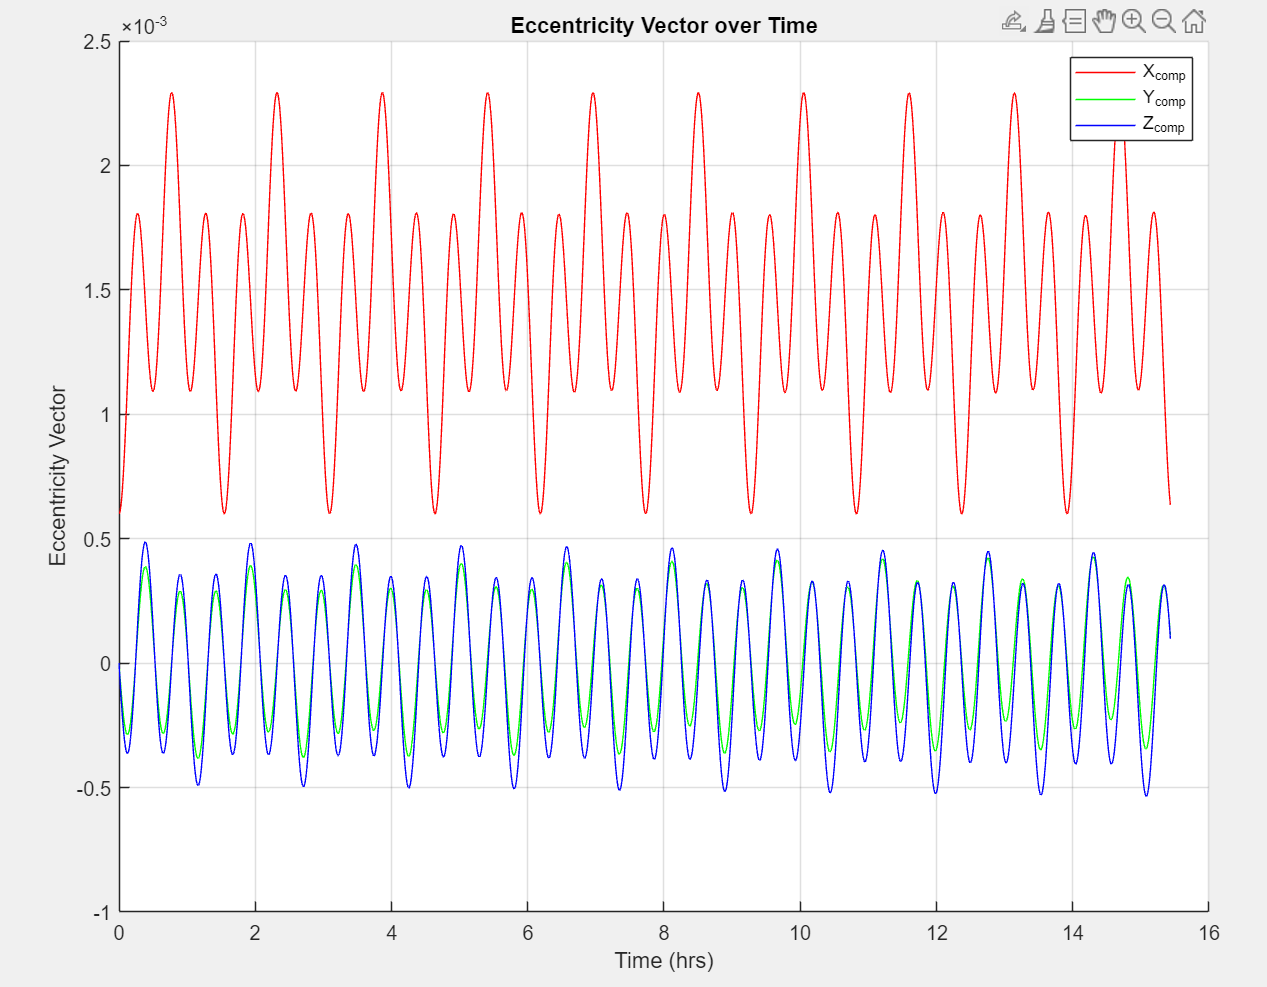
\includegraphics[width=0.5\textwidth]{PS1/Figures/eccentricity_vector_j2.png}
    \caption{Eccentricity vector components over time with J2 perturbation}
    \label{fig:ecc_vector}
\end{figure}

\begin{figure}[H]
    \centering
    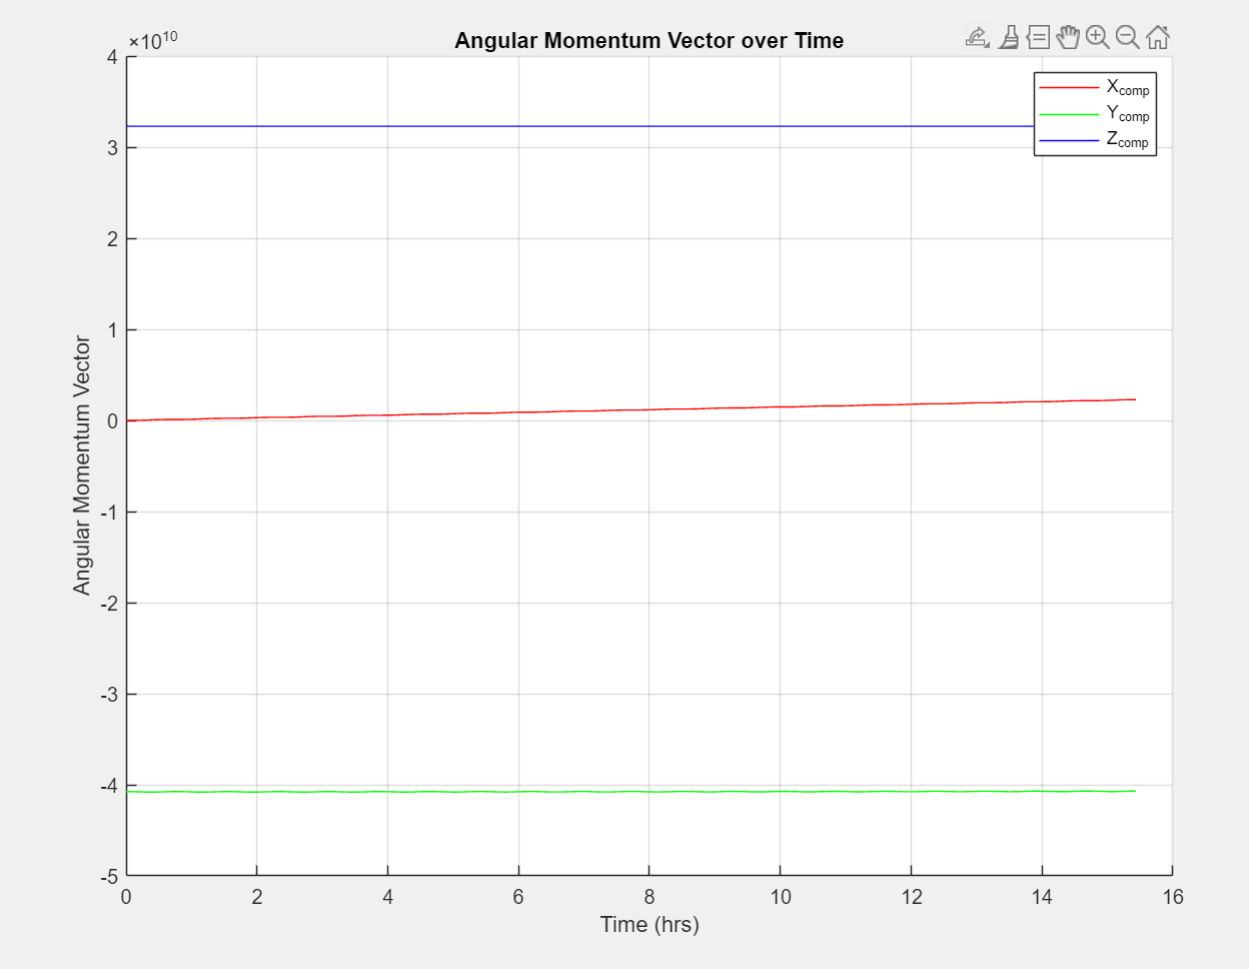
\includegraphics[width=0.5\textwidth]{PS1/Figures/angular_momentum_j2.png}
    \caption{Angular momentum vector components over time with J2 perturbation}
    \label{fig:ang_mom}
\end{figure}

\begin{figure}[H]
    \centering
    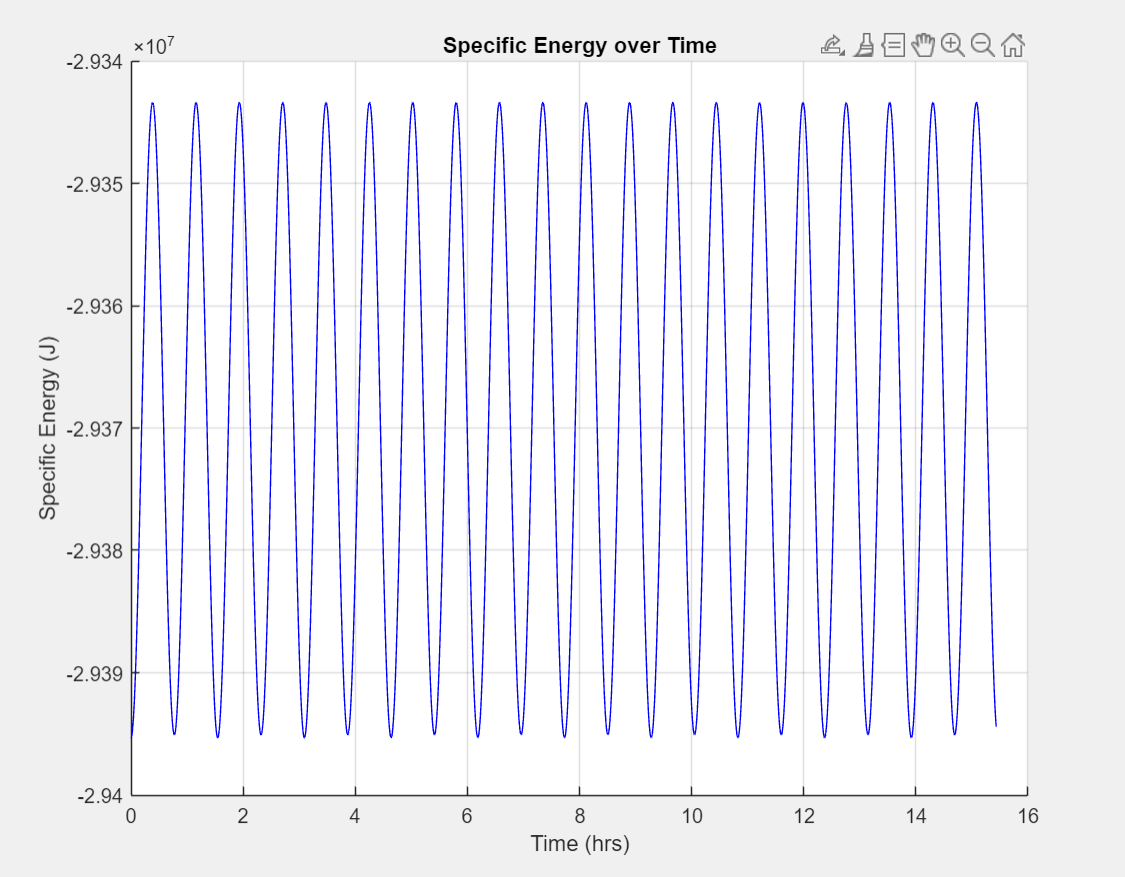
\includegraphics[width=0.5\textwidth]{PS1/Figures/specific_energy_j2.png}
    \caption{Specific mechanical energy over time with J2 perturbation}
    \label{fig:energy}
\end{figure}

In the unperturbed case (Figure \ref{fig:oe_unperturbed}), while we expect perfect conservation of orbital elements, some minor variations are observed due to numerical integration effects. In the J2-perturbed case (Figure \ref{fig:oe_j2}), semi-major axis and eccentricity show small oscillations but no secular trends, while RAAN and argument of periapsis exhibit clear secular drifts, with RAAN decreasing and argument of periapsis increasing. The angular momentum vector (Figure \ref{fig:ang_mom}) changes direction but maintains nearly constant magnitude.

\subsubsection{Mean Elements and Analytical J2 Effects}
In Figure \ref{fig:oe_j2}, the dashed lines show the analytical mean element solutions for RAAN and argument of periapsis. The mean elements follow linear trends that closely match the average behavior of the osculating elements, showing our J2 secular effects.

\subsubsection{Reconciliation of Osculating and Mean Elements}
To reconcile the difference between osculating and mean elements we must consider the fact that numerical integration takes in osculating elements, while the analytical solution to J2 takes in mean elements. Therefore, if the same inputs are used for both, the results will be slightly off. To fix this, the Brouwer transform could be applied to the starting elements.